\section{Micro-P4 \;($\mu$P4)}
Re-configurable targets process packets using multiple type of processing blocks and P4 provides multiple sub-languages following heterogenous abstract machines to program the blocks.
The presence of heterogeneous abstract-machines and device-specific constructs is the
primary reason for lack of mechanisms for modularity and code reuse.
Because, it is not possible to define interface to reuse code modules when caller and callee modules can have incompatible abstract machines.


$\mu$P4 comprise of an architecture, $\mu$SA, and a compiler, $\mu$P4C for a logical target device. 
$\mu$SA simplifies abstract machine for P4 data plane programs by exposing minimal number of programmable blocks required to implement.
It provides abstraction by defining logical externs that allows programmers to express packet-processing logic that is outside the scope of current P4 and relies on fixed-function blocks in real targets.
In $\mu$SA, we define generic interfaces to enable easy code reuse of fine-grained packet-processing functions and build new functions.
We associate runtime behavior with the generic interface as described in Section \ref{subsection:packet-processing-using-mp4}. 
$\mu$P4C allows programmer to express \emph{sequential} and \emph{parallel} execution multiple fine-grained functions.
Unlike Hyper4 and P4Visor, $\mu$P4C enables composition of packet-processing functions using P4 language itself without relying on different configuration languages.
It translates simplified abstract machine and its logical externs into real target-specific heterogeneous packet-processing blocks, features and constraints.


\subsection{Packet Processing using $\mu$P4}
\label{subsection:packet-processing-using-mp4}
We model every packet-processing function as a black-box micro-switch that processes packet byte-stream, intrinsic metadata and user-defined parameters as shown in Figure \ref{fig:package-runtime-behavior}.
The black-box model hides implementation details (headers types, user-defined metadata, programmable blocks etc.,) of micro-switch programs.
To realise this model, $\mu$SA defines multiple packet-processing pipelines and each pipeline is associated with one or more generic interface types.
Each generic interface exposes a set of programmable blocks to implement and allows programmers to specify type parameters for runtime arguments.
Programmers can implement the interfaces and define new \emph{package} types.
In control blocks of $\mu$SA pipelines, the package types can be instantiated and invoked by supplying arguments for the defined runtime parameters. 
\begin{figure}[!h]
    \centering
    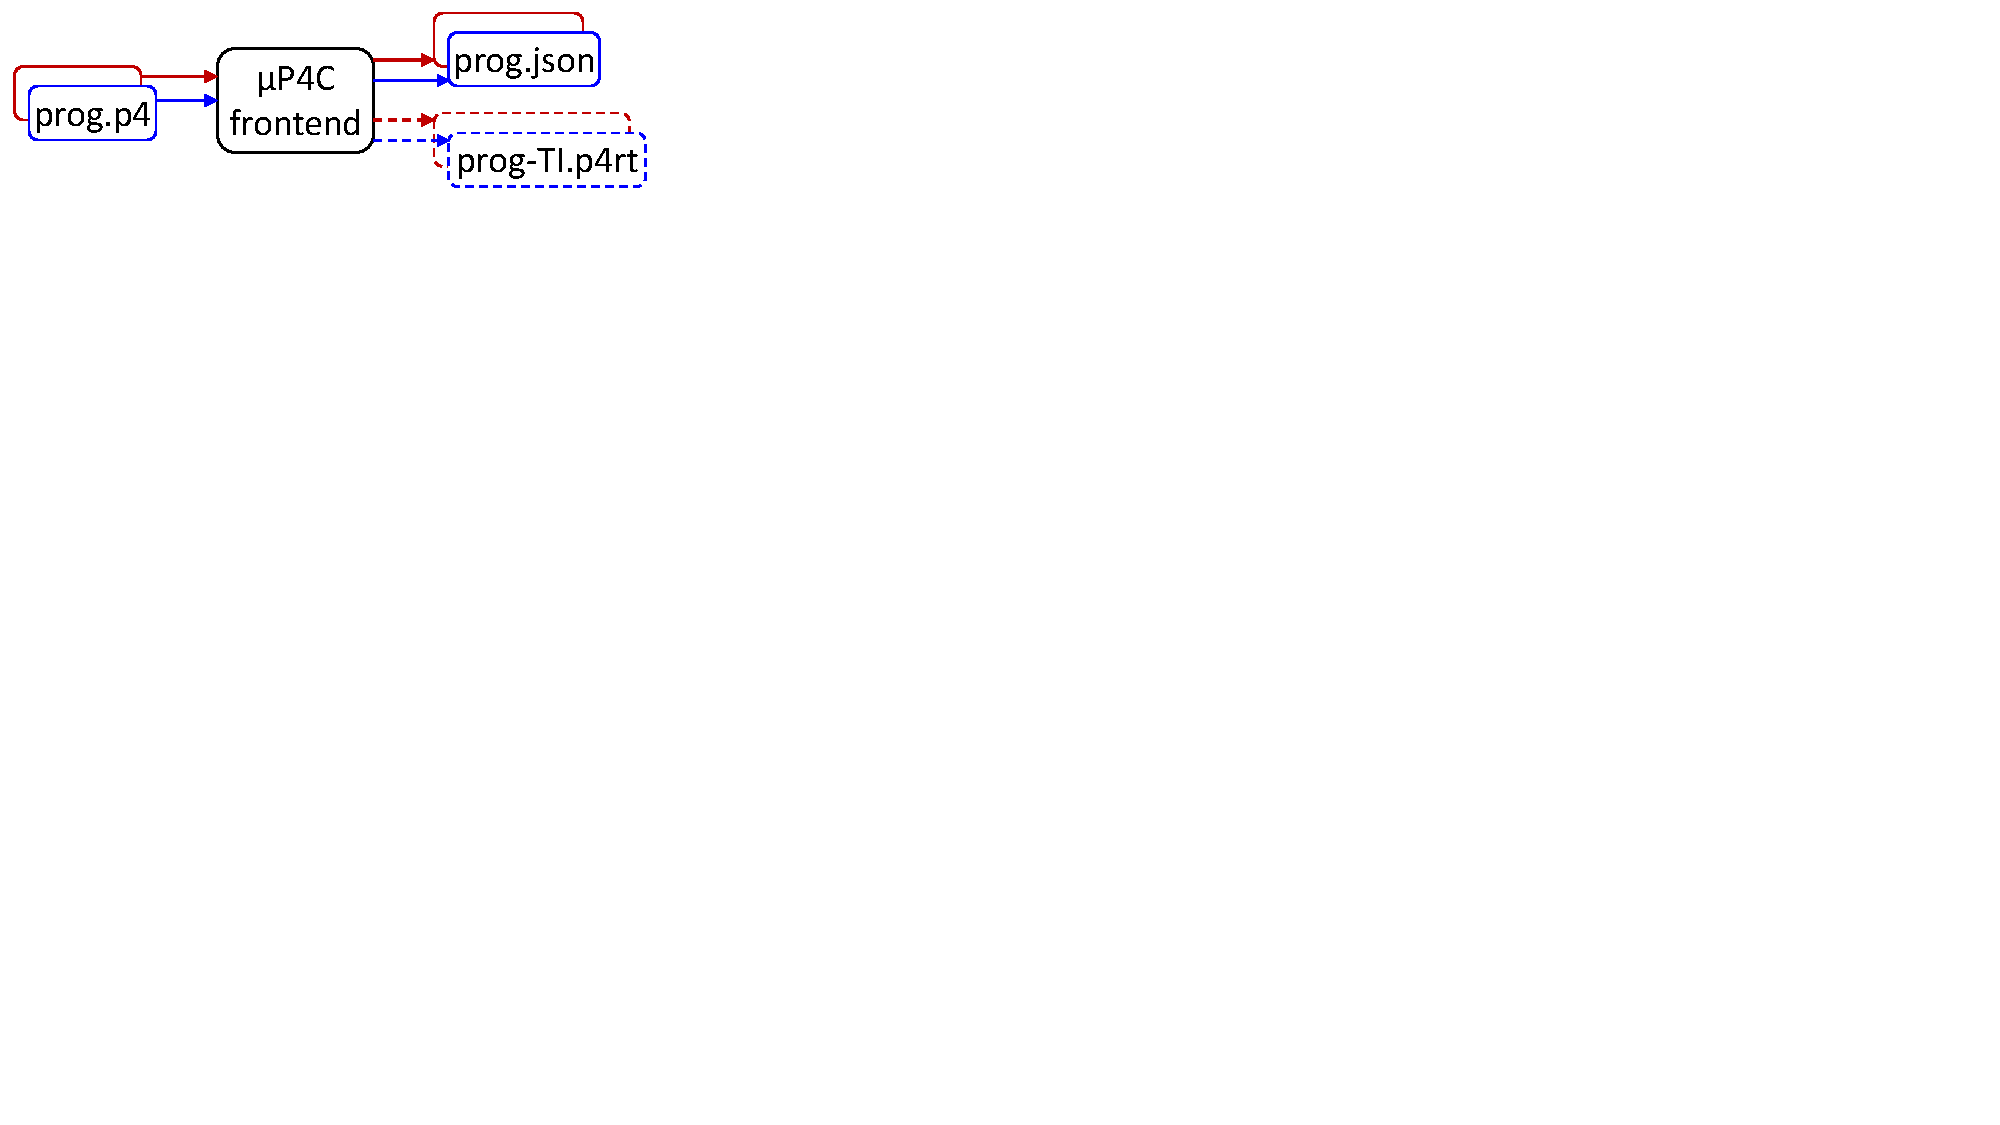
\includegraphics[trim=300 300 0 0, clip,scale=0.2]{mp4c-frontend}
    \caption{Micro P4 Package Runtime Behavior}
    \label{fig:package-runtime-behavior}
\end{figure}


\subsubsection{Sequential Execution}
Sequential execution of micro-switch programs follow a single-thread model.
Only one micro-switch program processes a packet at a time.
$\mu$P4 allows programmers to invoke micro-switch programs using their interfaces in body of control blocks other micro-switch program.
Programmers can logical externs defined in $\mu$SA to express sequential processing.
Figure \ref{fig:sequential-execution} extends the example of fine-grained functions described in \ref{fig:l3.p4.l2.p4}
 \begin{figure}[ht]
\begin{lstlisting}[frame=none]
// interfaces for l3 and l2
l3(pkt_in pi, pkt_out po, sm_t s, out bit<16> nh);
l2(pkt_in pi, pkt_out po, sm_t s, in bit<16> nh);

control (pkt_in pin, pkt_out po, sm_t s) {
  l3 l3_inst;  l2 l2_inst;  bit<16> next_hop;
  pkt_in pin_l2;
  apply {
    l3.apply(pi, po, s, next_hop);
    // sets `pin_l2' with `po's bytes, resets `po'
    po.get_pkt_in(pin_l2); // extern method call
    l2.apply(pin_l2, po, s, next_hop);
  }
}
\end{lstlisting}
\caption{Sequential Execution}
\label{fig:sequential-execution}
\end{figure}






\subsubsection{Parallel Execution}
In parallel execution, multiple micro-switch process a copy 

\subsection{Compiling $\mu$P4 programs}

% Third, we develop compiler mechanisms to have uniform abstract-machine for programmable blocks.
% Finally, we translate our unified abstract machine and logical externs into real target-specific heterogeneous packet-processing blocks, features and constraints.


% In this section, we present a system, $\mu$P4, comprising of an architecture, $\mu$SA for a logical target device and a compiler, $\mu$P4C, to compile $\mu$SA-specific code to real target-specific code.

% In section \ref{section:micros-awitch-architecture}, we explain the design of Micro Switch Architecture for a logical target that reduces number of programmable blocks and introduces logical externs to minimize heterogeneity in abstract model of P4 programs.







% What do we need to provide interface to code modules?
% 
% We need runtime behaviour with package. 
% packet, sm, es, inargs, inout args -> package -> packet, sm, es, out args, inout args
% P4 extended to 
% allow Define new Package types
% runtime behavior with package types
% 
% MicroP4 defines package interfaces.
% 
% 
% MicroP4 captures intrinsic metadata dependency of real targets using logical extern (egress\_spec)
% 
% MicroP4 defines common abstractions for target specific operations that can not be expressed in P4
% e.g., multicast




\begin{figure}[!h]
    \begin{subfigure}{\linewidth}
        \centering
        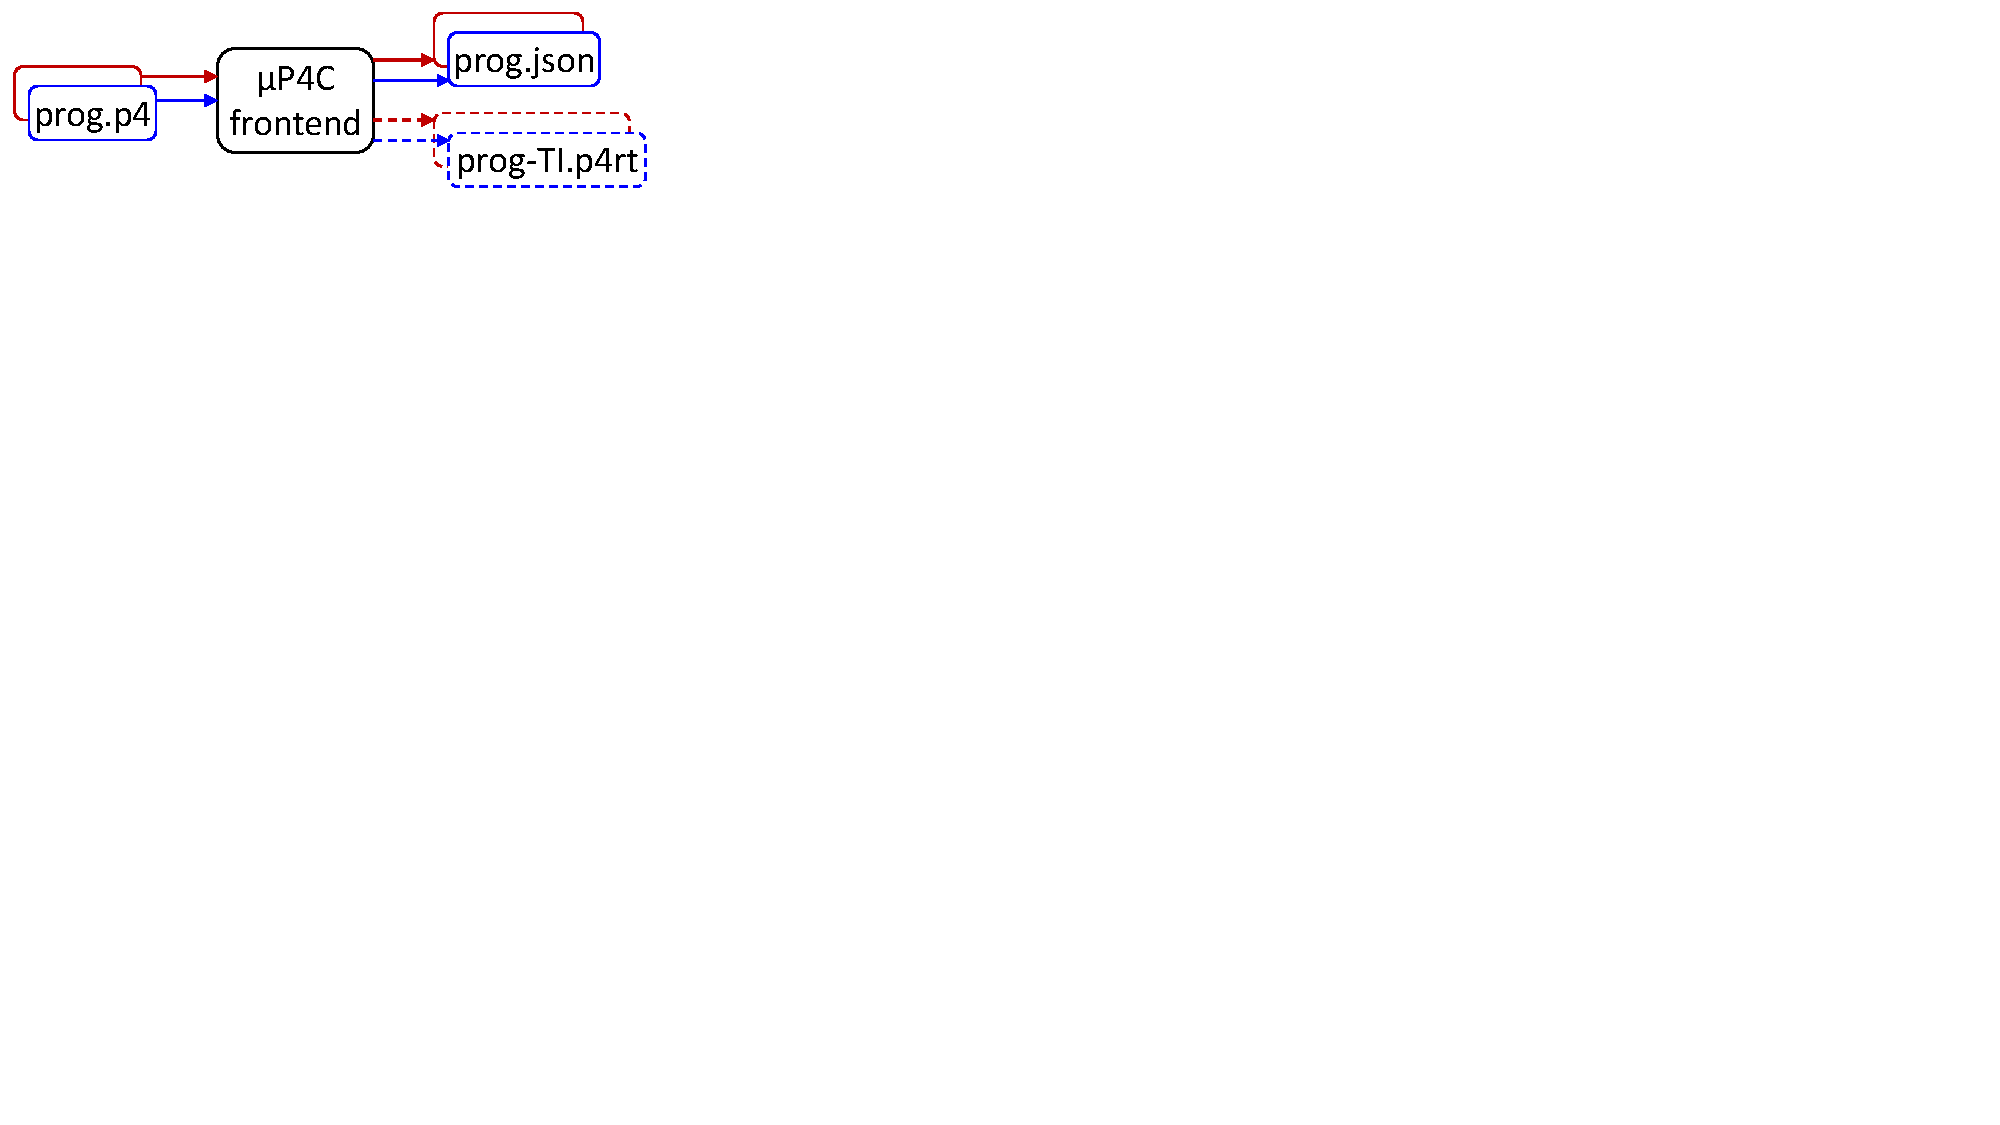
\includegraphics[trim=0 435 665 0, clip,scale=0.55]{mp4c-frontend}
        \caption{Library Program Compilation}
        \label{subfig:compiling-modules}
    \end{subfigure}
    \begin{subfigure}{\linewidth}
        \centering
        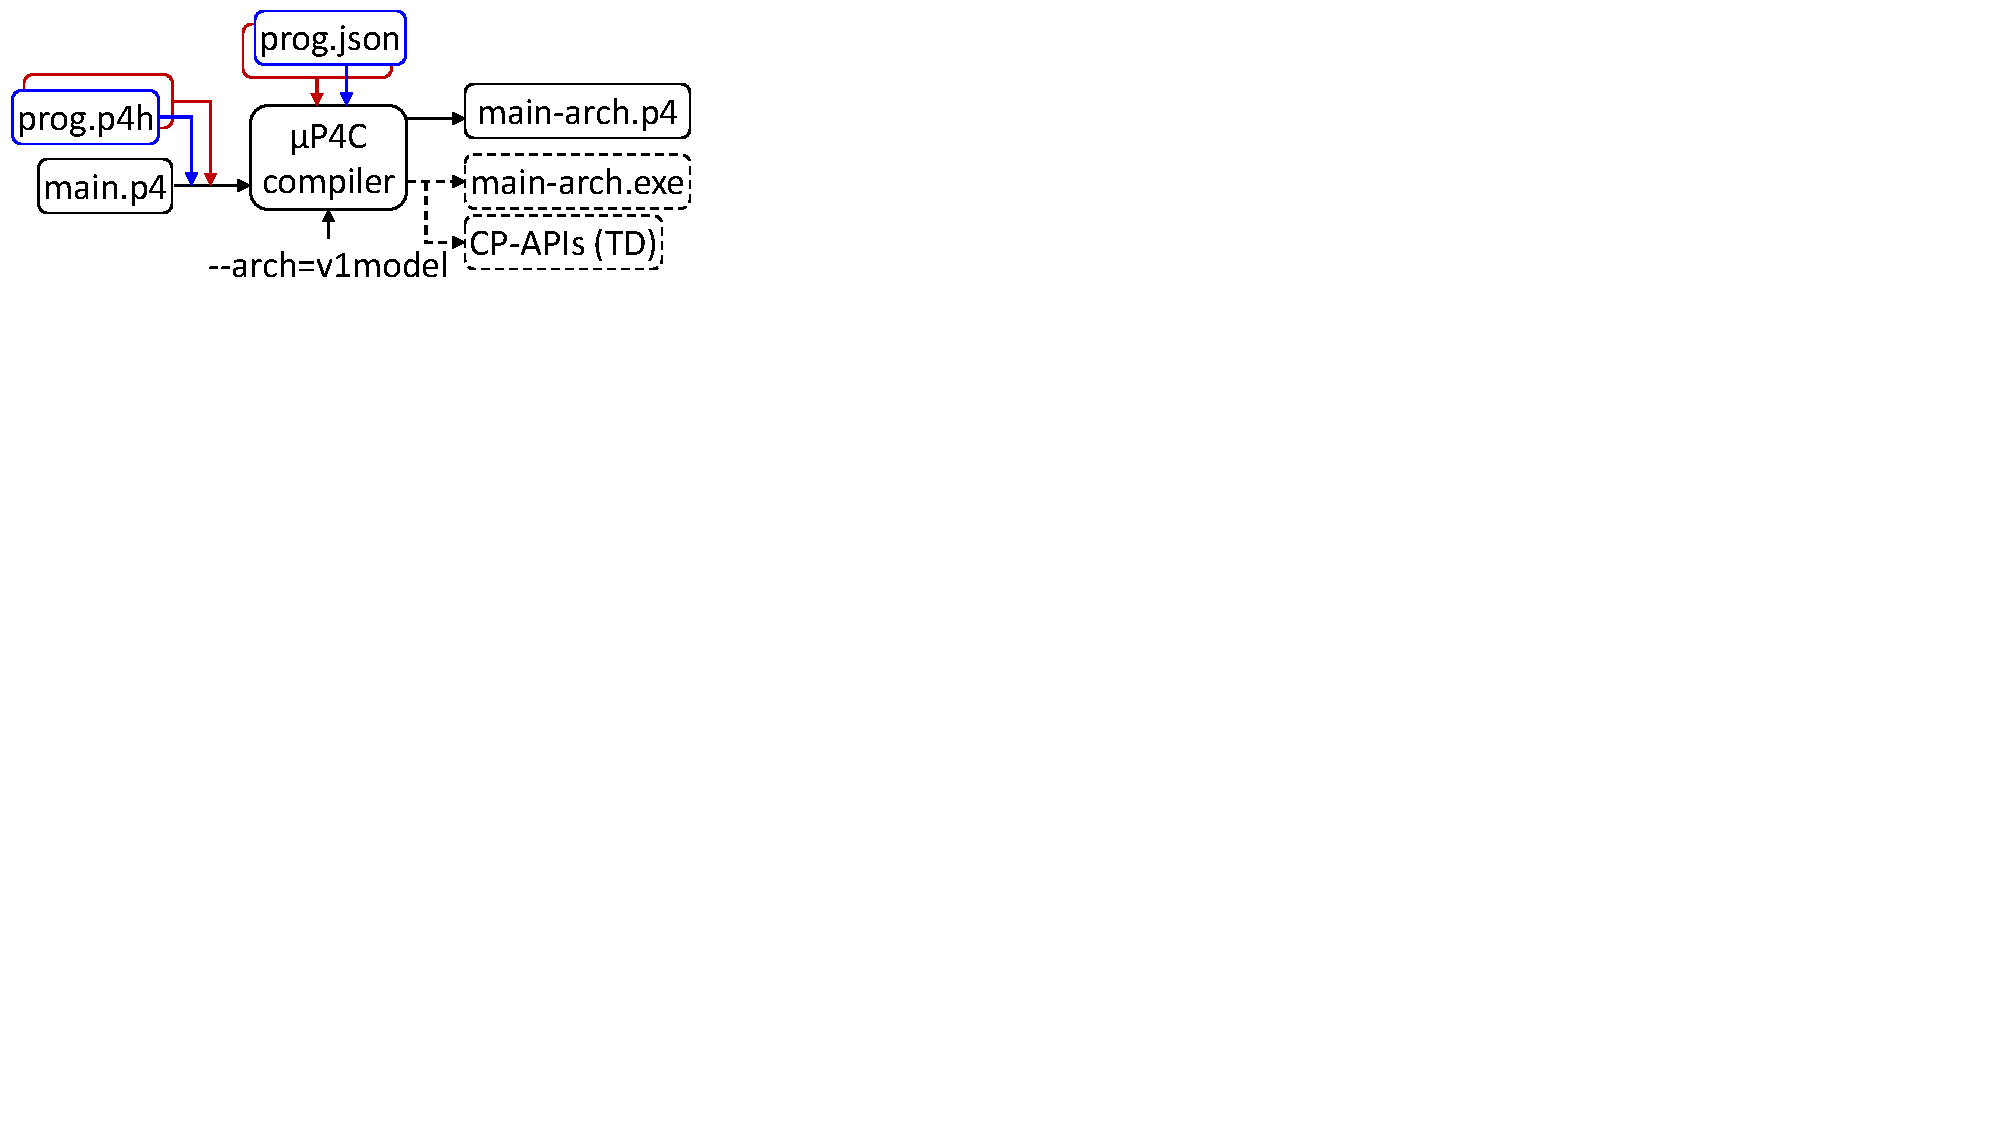
\includegraphics[trim=0 407 628 0, clip,scale=0.55]{mp4c-compiler}
        \caption{Composition and Translation of Main Instance}
        \label{subfig:composition-translation-of-main-instance}
    \end{subfigure}
\caption{Compiling $\mu$SA programs}
\label{fig:compiling-msa-programs}
\end{figure}
